% This is samplepaper.tex, a sample chapter demonstrating the
% LLNCS macro package for Springer Computer Science proceedings;
% Version 2.20 of 2017/10/04
%
\documentclass[runningheads]{llncs}
%
\usepackage{graphicx}
% Used for displaying a sample figure. If possible, figure files should
% be included in EPS format.
%
% If you use the hyperref package, please uncomment the following line
% to display URLs in blue roman font according to Springer's eBook style:
% \renewcommand\UrlFont{\color{blue}\rmfamily}
\usepackage{amsmath,amssymb}
\usepackage{amsfonts}
\usepackage{subfigure}

\begin{document}
%
\title{Wi-Fi Based Handwritten Signature Verification Using a Triplet Network}
%
\titlerunning{Wi-Fi Based Handwritten Signature Verification Using a Triplet Network}
% If the paper title is too long for the running head, you can set
% an abbreviated paper title here
%
\author{Young-Woong Kwon \and Jooyoung Kim \and Kar-Ann Toh}
%
\authorrunning{Y. Kwon et al.}
% First names are abbreviated in the running head.
% If there are more than two authors, 'et al.' is used.
%
\institute{
School of Electrical and Electronic Engineering, Yonsei University, 50 Yonsei-ro, Seodaemun-gu, Seoul 03722, Republic of Korea\\
\email{\{herokwon, harrykim, katoh\}@yonsei.ac.kr}}
%
\maketitle              % typeset the header of the contribution
%
\begin{abstract}
%The abstract should briefly summarize the contents of the paper in 15--250 words.
In this paper, we propose a system for identity verification based on the handwritten signature signals captured by the Wi-Fi Channel State Information (CSI). 
To enable a fast loss convergence, a kernel and the range space learning is initially adopted for refining the triplet inputs by mining the distinctive inputs. 
Subsequently, the triplet network is trained on a ConvNet structure using the mined triplet inputs. 
Our experiments on an in-house Wi-Fi handwritten signature signal dataset show encouraging verification accuracy with faster training loss convergence comparing with the baseline triplet network and the Siamese network.

\keywords{Wi-Fi signature signal \and in-air handwritten signature verification \and the Kernel and the Range space projection learning \and triplet network}
\end{abstract}
%
%
%
\section{Introduction}

Over recent years, several behavioral biometric traits attracted attention in view of their rigid physical body independence~\cite{bailador2011analysis}. Among these behavioral biometrics, the signature-based user authentication~\cite{sanmorino2012survey,galbally2015line} has attracted considerable interest with the development of in-air signature recognition systems~\cite{jeon2012system,sesa2012information,malik20183dairsig}.
With the help of sensors such as the depth camera~\cite{malik20183dairsig} or a mobile sensor~\cite{jeon2012system}, the in-air signature recognition system has lower the spatial constraint in the process of signature acquisition comparing with contact-based authentication systems. 

Recently, the commercial Wi-Fi device has been adopted for in-air signature authentication due to its easy accessible property \cite{moon2017air}. Based on the distortion of the  Wi-Fi CSI signal according to the user's gestures, the in-air signature recognition system showed reasonable user verification performance~\cite{moon2017air}. More recently, some studies attempted to implement the deep learning algorithms in Wi-Fi signal-based user authentication systems to improve the verification performance ~\cite{shi2017smart,pokkunuru2018neuralwave}. 

In this paper, we utilize the deep triplet network for identity verification based on the Wi-Fi CSI signature signal. To achieve not only the desired verification accuracy but also a fast training speed, we adopt the kernel and the range (KAR) space learning~\cite{toh100,toh2018learning,toh2018analytic,toh2018gradient} in order to mine the distinctive triplet inputs. Subsequently, the triplet network which utilizes the ConvNet structure as a feature extractor is trained based on the L-2 distance comparison.

The main contributions of our work can be summarized as follows:
\begin{itemize}
\item Proposal of a system for identity verification based on the Wi-Fi handwritten signature signals using a deep triplet network.
\item Adopted the kernel and the range (KAR) space learning in order to mine the distinctive triplet inputs which boost the convergence speed of the training loss in the triplet network.
\item Provision of an experimental study using an in-house Wi-Fi handwritten signature dataset collected from 50 subjects.
\end{itemize}

The paper is organized as follows: related works including the triplet network and KAR space learning are introduced in Section 2 for immediate reference. Our proposed method are discussed in Section 3. Section 4 describes our experimental results and analysis. Some concluding remarks are given in Section 5.


\section{Related works}

\subsection{Triplet network}
% triplet network
The triplet network is considered a metric learning based model~\cite{weinberger2006distance} which aims to learn useful representations by means of distance comparison~\cite{hoffer2015deep}. 
It is often seen in person re-identification~\cite{chen2017beyond,cheng2016person,ding2015deep,schroff2015facenet,wang2016joint} where the individual identities are matched based on discriminative image features. The main difference between person identification and re-identification is that the later is a more challenging task where images of the same person taken from different cameras or from the same camera in different occasions are to be associated. In this re-identification problem, to distinguish among the classes is a challenging task since the features are relatively weak compared with the background features. To address this problem, we adopt a triplet network which optimizes the embedding data space so that data points with the same identity are closer to each other than those with different identities~\cite{hermans2017defense}.

The triplet network receives triplet pairs of data as its input. These data triplets are constructed based on a combination of the input data. Since not all triplet samples contribute to the desired classification, recent attention~\cite{schroff2015facenet} has been paid to the choice of relevant input pairs for training. In order to optimize the training process which utilizes only some parts of the triplet pairs, several researches~\cite{cheng2016person,ding2015deep,wang2016joint} generated triplet from a small number of classes (persons) in each iteration. Recently, \cite{schroff2015facenet} adopted a triplet mining process to speed up the training convergence. They utilized a large mini-batch at each training iteration and selected the triplet based on the training network rather than random sampling. However, this strategy needed a few thousands of exemplar mini-batches in every training iteration for triplet pairs selection. This results in a heavy computational load in training.

% Rel works: KAR learning
\subsection{Kernel and the range space learning~\cite{toh100,toh2018learning,toh2018analytic,toh2018gradient}}\label{kar}

Generally, the multilayer feedforward neural networks is trained based on the gradient descent method via backpropagation~\cite{goodfellow2016deep}.
However, setting the learning parameters such as the learning rate or the learning momentum is a time consuming task.

Recently, a gradient-free learning framework based on the kernel and the range (KAR) space manipulation has been developed for multilayer network learning~\cite{toh2018learning,toh2018gradient}.
The learning method is grounded on linear algebra with neither learning parameters nor iteration is needed in training.

% Karnet structure and mining samples.
Given $m$ training samples. Let $\mathbf{X}\in{\mathbb{R}}^{m \times (n+1)}$ denotes the training data set and $\mathbf{G}\in{\mathbb{R}}^{m \times n}$ denotes the network outputs.
Then the multilayer neural network structure can be written in linear equation form as follows:
\begin{equation}
    \mathbf{G} = \sigma\left(\left[\mathbf{1},\sigma\left(\dots\left[\mathbf{1},\sigma\left(\left[\mathbf{1},\sigma\left(\mathbf{X}\mathbf{W}_{1}\right)\right]\mathbf{W}_{2}\right)\right]\dots\mathbf{W}_{(i-1)}\right)\right]\mathbf{W}_{i}\right), i=1,\dotsc,n,
\end{equation}
where $\mathbf{W}_{1}\in{\mathbb{R}}^{(n+1) \times h_{1}}$,$\mathbf{W}_{2}\in{\mathbb{R}}^{(h_{1}+1) \times h_{2}}$,$\dots,\mathbf{W}_{i}\in{\mathbb{R}}^{(h_{(i-1)}+1) \times n}$,$\mathbf{1}=\left[1,\dots,1\right]^{T}\\
\in{\mathbb{R}}^{m \times 1}$ and $\sigma(.)$ is the activation function.
By adopting an one-hot encoded target $\mathbf{Y}\in{\mathbb{R}}^{m \times n}$, training of the weight matrices $\mathbf{W}_{i}$ using the KAR space method~\cite{toh2018gradient} can be computed as follows:

\begin{equation}
    \mathbf{W}_{i} = \left[\mathbf{1},\sigma\left(\dots\left[\mathbf{1},\sigma\left(\left[\mathbf{1},\sigma\left(\mathbf{X}\mathbf{W}_{1}\right)\right]\mathbf{W}_{2}\right)\right]\dots\mathbf{W}_{(i-1)}\right)\right]^{\dagger}\sigma^{-1}\left(\mathbf{Y}\right), i=1,\dotsc,n.
\end{equation}

%% Methods
\section{Proposed System}

% Methods: System overview(Fig.1)
In this section, we propose an identity verification system based on the Wi-Fi in-air handwritten signature (which will be called Wi-Fi signature hereafter) using the triplet network~\cite{hoffer2015deep}. Fig.1 shows an overview of the proposed system utilizing the kernel and the range (KAR) space learning~\cite{toh2018learning,toh2018gradient} for mining the triplet input.
Essentially, the KAR space projection learning is utilized to learn the triplet input data by mining the hard positive and the hard negative samples from each given anchor sample (see item (a) in Fig.~\ref{fig1}). The hard positive and the hard negative samples refer to positive and negative class samples which are likely to be misclassified by the network.
Subsequently, the ConvNet structure in the triplet network (see item (b) in Fig.~\ref{fig1}) is trained with the mined triplet data based on a triplet loss function using the L-2 distance comparison (see item (c) in Fig.~\ref{fig1}).
The following subsections describe the details of the triplet mining using KAR space learning and the triplet network.

% Figure 1
\begin{figure}[!ht]
    \includegraphics[width=\textwidth]{fig1_tcnn_kar_v5}
    \caption{An overview of the proposed system.} \label{fig1}
\end{figure}

% Methods: KAR learning
\subsection{Triplet mining using kernel and the range space learning}

The network receives a triplet set of data as its inputs. These triplet data consist of the reference data (will be called anchor samples hereafter) and the corresponding positive class data (same class with that of the anchor) and negative class data (different class from that of the anchor). The goal of the triplet network is to position the feature vectors with appropriate separation space by putting the positive samples close to the anchor sample and keeping the negative sample away from the anchor sample.

According to \cite{schroff2015facenet}, it is important to select the hard positive samples and the hard negative samples with reference to the given anchor sample for fast loss convergence when training the triplet network.
A hard positive sample is defined as a sample whose distance to the anchor sample is large (which is most likely to be misclassified as a negative sample). On the other hand, a hard negative sample is defined as a sample whose distance to the anchor sample is small (which is most likely to be misclassified as a positive sample). However, from the raw data, there is no information about regarding whether a sample is considered hard positive or hard negative before we train the network.

In this work, we propose to adopt the kernel and the range (KAR) space learning (see Section~\ref{kar} for details) as a pretraining network to mine the hard positive/negative samples from the given anchor sample. Since the KAR space learning has no iterative learning process, we can mine the triplet samples without using the time consuming backpropagation training process.
 
By training the network with the single shot KAR space learning, we can map the L-2 distance between every samples by using the output vector of the KAR space network. \textbf{For training dataset $\mathbf{X}$, the trained network output is given by:}
\begin{equation}
    f\left(\mathbf{X}\right) = \sigma\left(\left[\mathbf{1},\sigma\left(\dots\left[\mathbf{1},\sigma\left(\left[\mathbf{1},\sigma\left(\mathbf{X}\cdot\mathbf{W}_{1}\right)\right]\mathbf{W}_{2}\right)\right]\dots\mathbf{W}_{(i-1)}\right)\right]\mathbf{W}_{i}\right),
\end{equation}
\textbf{For anchor sample $\mathbf{x}_{anc}$ which is randomly selected from training dataset X, the output of the KAR learning makes it possible to measure the distance between each sample.}
A hard positive sample $\mathbf{x}_{pos}$ and a hard negative sample $\mathbf{x}_{neg}$ with respect to the anchor sample $\mathbf{x}_{anc}$ can each be respectively determined based on:
\begin{equation}
    {\left\| {{f\left(\mathbf{x}_{anc}\right)} - {f\left(\mathbf{x}_{pos}\right)}} \right\|_2^2} \geq \mathrm{t}_{pos}, \label{pos}
\end{equation}
\begin{equation}
    {\left\| {{f\left(\mathbf{x}_{anc}\right)} - {f\left(\mathbf{x}_{neg}\right)}} \right\|_2^2} \leq \mathrm{t}_{neg},\label{neg}
\end{equation}
where $\mathrm{t}_{pos}$ and $\mathrm{t}_{neg}$ respectively denote the thresholds that determine whether a sample is hard positive or hard negative. Since the hardest samples are likely to be outliers which can degrade the training process of the triplet network, we empirically set the $\mathrm{t}_{pos}$ at 75 percentile of the L-2 distance and $\mathrm{t}_{neg}$ at 25 percentile of the L-2 distance. The final set of $\mathbf{x}_{pos}$ and $\mathbf{x}_{neg}$ samples is randomly selected from those samples threshold by~\eqref{pos} and~\eqref{neg}.

% Methods: ConvNets
\subsection{ConvNet structure}

The next step is to design a feature extractor which converts the input triplet data into feature vectors. In this work, we utilize the ConvNet structure~\cite{lecun1998gradient} as a feature extractor since the three-dimensional data format of our preprocessed input signal can be regarded as an image data format with multiple channels. 

Our ConvNet structure (item (b) in Fig~\ref{fig1}) for the network consists of three convolutional layers and one fully-connected layer. The number of convolutional filters to be trained in each layer is empirically chosen as $\{64, 128, 256\}$, with fixed filter size of $3\times3$, each of stride 1. The Rectified Linear (ReLU) activation function and the Max-pooling layer are applied between each convolutional layer. Subsequently, the extracted features from the last convolutional layer are flattened into a vector before feeding into the fully-connected network.
The output vectors from the fully-connected layer are finally transformed using the sigmoid function followed by a L-2 normalization.

% Methods: Triplet loss
\subsection{The triplet loss}

The triplet loss function was first seen in \cite{hoffer2015deep} for training the triplet network.
\textbf{For selected anchor input sample $\mathbf{x}_{anc,i}$, the $i_{th}$ triplet input $\left\{\mathbf{x}_{anc,i}, \mathbf{x}_{pos,i}, \mathbf{x}_{neg,i}\right\}$ is generated by grouping positive input sample $\mathbf{x}_{pos,i}$ and the negative input sample $\mathbf{x}_{neg,i}$.
The generated triplet input is fed into ConvNet structure and make feature vectors $\left\{\mathbf{v}_{anc,i},\mathbf{v}_{pos,i},\mathbf{v}_{neg,i}\right\}$.}
The triplet loss function is formulated based on a summation of the difference between the positive distance (the L-2 distance between the anchor vector and the positive vector) and the negative distance (the L-2 distance between the anchor vector and the negative vector) as follows:
\begin{equation}
    loss = \sum_i^N max\left({ \left[ {\left\| {{\mathbf{v}_{anc,i}} - {\mathbf{v}_{pos,i}}} \right\|_2^2} - {\left\| {{\mathbf{v}_{anc,i}} - {\mathbf{v}_{neg,i}}} \right\|_2^2}  + \alpha \right]}, 0 \right),\label{triplet}
\end{equation}
where $N$ denotes the size of the mini-batch, ${\left\| . \right\|_2^2}$ denotes the L-2 distance and $\alpha$ denotes the preset margin.
The ConvNet structure using equation~\eqref{triplet} is trained to maximize the gap between the positive distance and the negative distance which should be larger than the margin $\alpha$.

\section{Experiments}

% Dataset
\subsection{Dataset}
 In order to evaluate the verification performance of the proposed system, the Wi-Fi CSI signature dataset \cite{moon2017air} with the user located at a single position is utilized in our experiments. The Wi-Fi CSI signature dataset consists of 2000 Wi-Fi CSI signature signals (4 directions $\times$ 10 samples $\times$ 50 identities) with sample size 500$\times$30$\times$6. We utilize only the absolute value from each complex CSI signal in our experiments.

\subsection{Experimental settings}

\subsubsection{Performance evaluation:}
The proposed system is evaluated under two cases: i) case I on comparison between the proposed system and other handcraft or deep learning-based methods based on the verification accuracy, and case II on detailed comparison between the proposed system and the deep learning-based methods using the receiver operating characteristic (ROC) curve and training loss curve. For Case I, existing handcraft methods such as the least squares error estimation (LSE), the principal components analysis (PCA) [22] with LSE, the support vector machine (SVM) with different kernel functions and a total error rate minimization which adopted the reduced multivariate polynomial model as basis function (TER-RM2) \cite{toh2003fingerprint,toh2008between}, the deep learning-based Siamese network \cite{koch2015siamese} and the baseline triplet network \cite{hoffer2015deep} are included for performance benchmarking. The Siamese network and the baseline triplet network utilized the same ConvNet structures with the proposed system and only differed in their input data style and loss function.

The verification performance of the proposed system and other methods are evaluated in terms of the Equal Error Rate (EER, \%) which are taken from averaging the results of five runs of two-fold cross-validation tests. Due to the memory constraint caused by the large data size, the deep learning-based methods utilized randomly sampled 9,500 negative pairs in the validation stage, which is the same number as the number of positive pairs.

\subsubsection{Network Structure and Parameter Settings:}
The multilayer feedforward network structure of KAR space learning is specified in Table~\ref{tab2}. With input data, size of 500$\times$30$\times$6, we set two network layers where the size of the each layer is 1024 and 16, respectively. Each layer is initialized with uniform distribution over [0, 1). We used $\sigma = {tan}^{-1}$ as an activation function following \cite{toh2018analytic}.

\begin{table}[]
    \caption{The network structure of KAR space learning.}\label{tab2}
    \centering
    \begin{tabular}{|l|l|l|}
    \hline
    Layer   & Size     & Activation \\ \hline
    Input   & 500$\times$30$\times$6 &            \\
    Fully-Connected 1 & 1$\times$1$\times$1024 & $\sigma = {tan}^{-1}$     \\
    Fully-Connected 2 & 1$\times$1$\times$16  & $\sigma = {tan}^{-1}$     \\
    Output  & 1$\times$1$\times$50   &            \\ \hline
    \end{tabular}
\end{table}

For the proposed system and the deep learning-based methods, we utilized the same ConvNet structure as specified in Table~\ref{tab1}. We trained the network starting with a learning rate of 0.00005 and a mini-batch size of 32. We optimized the loss by the Adam optimizer with L-2 penalty of 0.0002 except for the output layer. The output layer was regularized using an L-2 penalty of 0.0001. We initialized all network weights in the convolutional layers with normal distribution of zero-mean and standard deviation of 0.01. The biases were also initialized with a normal distribution of 0.5 mean and standard deviation 0.01. For the triplet networks, the hyper-parameter regulating triplet loss is empirically set at 0.1. The training epochs were set at 1,500 for all three deep learning-based algorithms. For the linear methods such as LSE,SVM and TER, the input signals were resized to 500 $\times$ 30 by averaging along the subcarrier axes due to limitation of hardware memory. For the PCA-LSE, the input dimension was reduced to 40.
 \begin{table}[]
    \caption{
        The structure of ConvNet model. For the convolution layer, kernel is specified as (m$\times$m) sized filter $\times$ \# of filters / \# of stride. For the max-pooling layer, (p$\times$p) sized pooling windows / \# of stride. The input sizes are denoted as rows $\times$ cols $\times$ \# of filters. 
    }\label{tab1}
    \centering
    \begin{tabular}{|c|c|c|c|}
    \hline
    Layer     & Activation & Kernel / Stride & Input Size \\ \hline
    Conv 1    & ReLU       & (3$\times$3)$\times$64/1      & 500$\times$30$\times$6   \\
    MaxPool 1 &            & (2$\times$2)/1         & 500$\times$30$\times$64  \\
    Conv 2    & ReLU       & (3$\times$3)$\times$128/1     & 250$\times$15$\times$64 \\
    MaxPool 2 &            & (2$\times$2)/1         & 250$\times$15$\times$128 \\
    Conv 3    & ReLU       & (3$\times$3)$\times$256/1     & 125$\times$8$\times$128  \\
    MaxPool 3 &            & (2$\times$2)/1         & 125$\times$8$\times$256  \\
    Fully-Connected     & Sigmoid    & 16             & 63$\times$4$\times$256   \\
    L-2 Norm  &            &                 & 1$\times$1$\times$16    \\
    Concat    &            &                 & 1$\times$1$\times$16    \\ \hline
    \end{tabular}
\end{table}

\subsection{Results and discussion}

Case I: Table~\ref{tab3} shows the best average of EER performance from five runs of two-fold cross-validation test and the parameter condition. Among the handcraft methods, the SVM with RBF kernel showed the best verification accuracy of 24.31\% EER followed by the SVM with Linear kernel function. However, all three deep learning-based methods showed better performance than the SVM with RBF kernel function since the deep learning-based methods could utilize the original size (500$\times$30$\times$6) of the input data in the training stage.
Among the deep learning-based methods, the Siamese network is also a metric learning system, but it differs from our system in that it receives two inputs and uses the contrastive loss function for training. 
The best average of test EER performance was obtained from the proposed system with 19.35\% EER. The baseline triplet network without input mining showed slightly worse performance of 20.34\% EER. The Siamese network showed the worst verification performance of 23.53\% EER.
\begin{table}[!h]
    \caption{Performance benchmarking with respect to the best EER (\%) averaged from five runs of two-fold cross-validation test on Wi-Fi CSI signature dataset.}\label{tab3}
    \centering
    \begin{tabular}{|c|c|c|}
    \hline
    Methology   &   Best EER (\%) &   Condition   \\  \hline
    LSE &   48.44   &  - \\ 
    PCA-LSE    &   30.79   &  Reduced dimension=40    \\
    SVM (Linear) &   28.23   &   c=1 \\
    SVM (RBF)    &   24.31   &   c=1, $\gamma$=0.01/3000 \\
    TER-RM2 &   35.84   &  M=1,$\tau$=$\eta$=0.5   \\     \hline
    Siamese network  &   23.53   &   lr=0.00005  \\
    Baseline triplet network &   20.34   &   lr=0.00005, $\alpha$=0.1  \\
    \textbf{Proposed system} &   \textbf{19.35}   &  \textbf{lr=0.00005, $\alpha$=0.1}  \\
     \hline
    \end{tabular}
\end{table}
Case II: Fig.~\ref{fig2}(a) shows the ROC curve of three deep learning-based methods. As shown in the Fig.~\ref{fig2}(b), the proposed system clearly shows the largest Area Under Curve (AUC) among three compared methods while other two methods show similar AUC. Moreover in Fig.\ref{fig2}(b) which illustrates the training loss curve along the number of training iteration, the proposed system shows the fastest training loss convergence followed by the baseline triplet network. We note here that the y-axes of triplet network based methods and the Siamese network are normalized into $[0,1]$ since each loss function has different starting value based on their function. According to these two observations, it can be concluded that the triplet input mining with KAR space learning improves not only the training loss convergence speed but also the verification performance.

% Figure 2,3
\begin{figure}[!ht]
    \begin{center}
    \subfigure[][ROC Curve]{
        \includegraphics[height=6.4cm]{fig_roc_v11.eps}}
    \subfigure[][Normalized training loss curve]{
        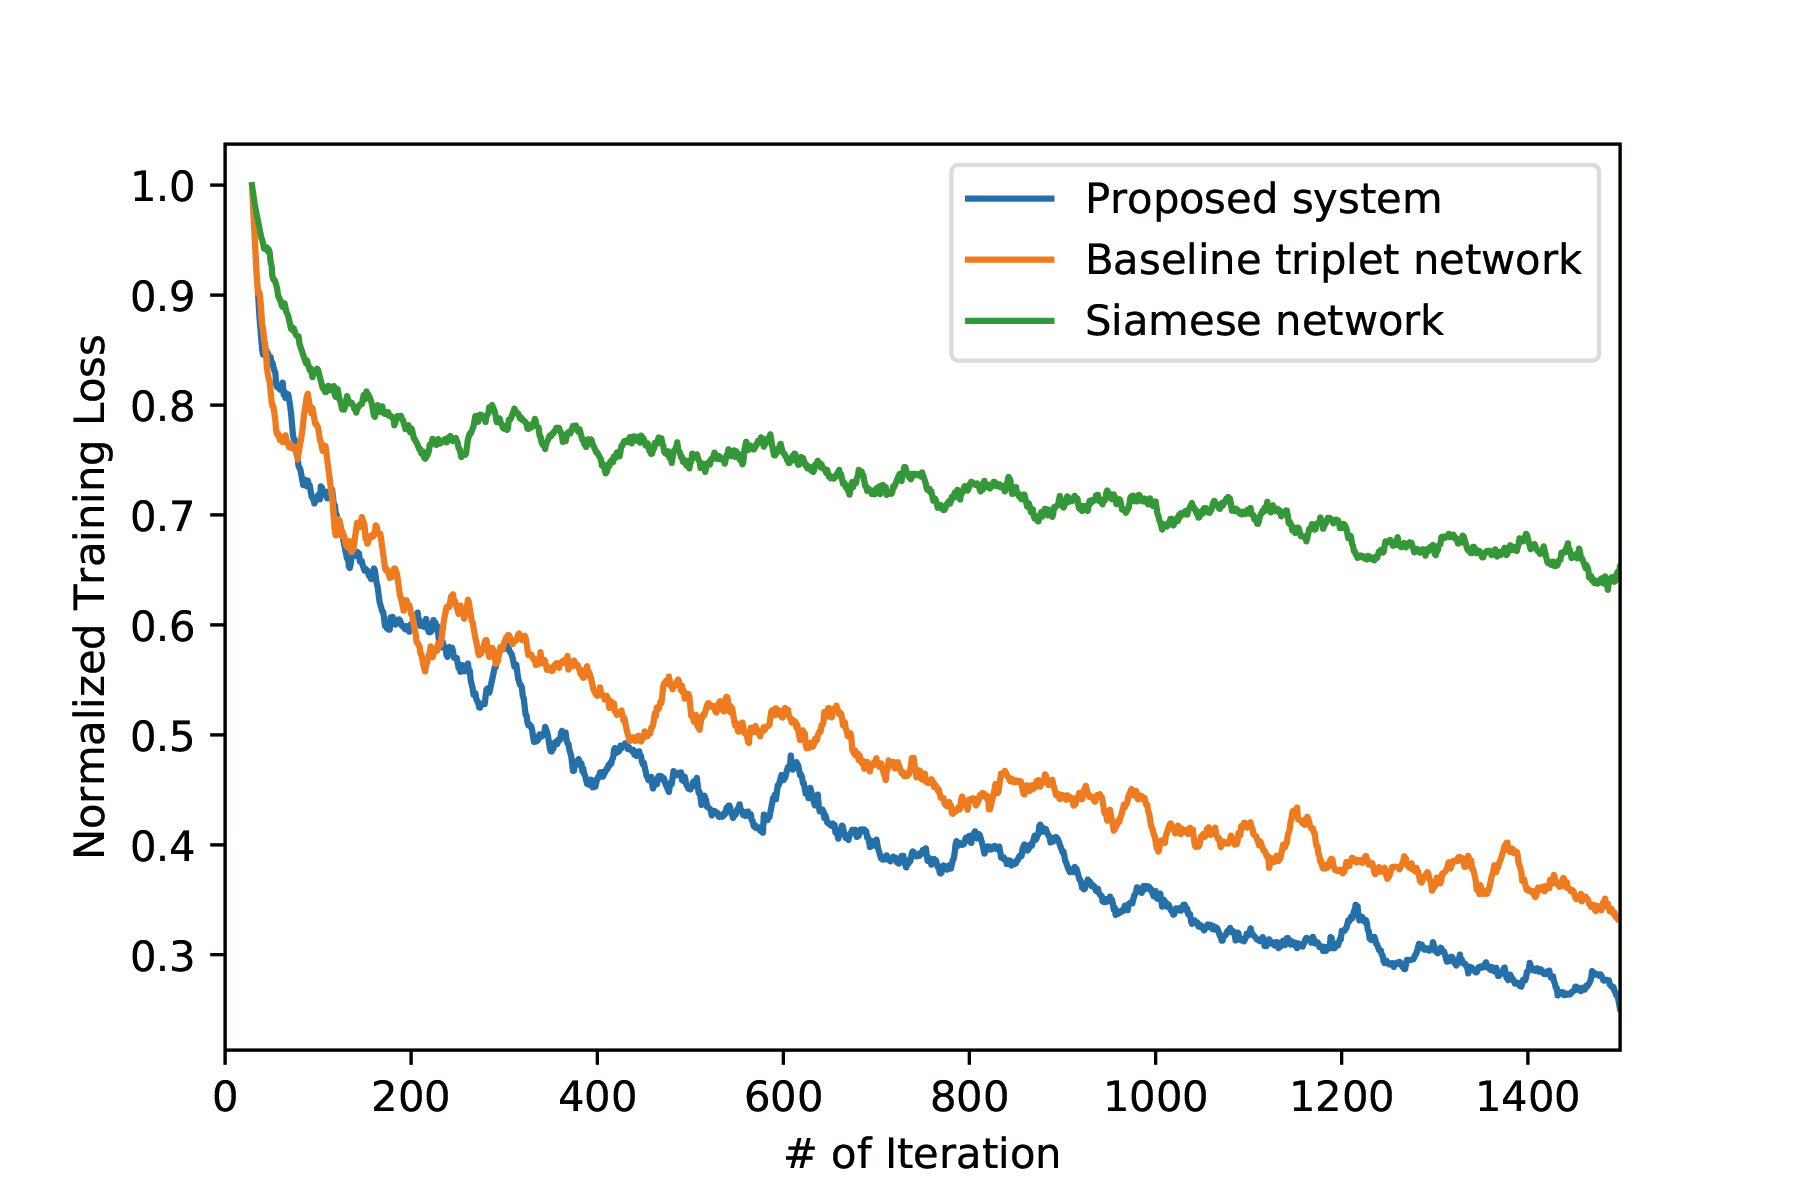
\includegraphics[height=6.4cm]{normalized_loss_curve_ma30_v2.eps}}
    \caption{(a) shows the Receiver Operating Characteristic(ROC) Curve and 
    (b) shows the normalized training loss curve of the deep learning based methods. }
    \label{fig2}
    \end{center}
 \end{figure}

\section{Conclusion}
In this paper, we proposed a system for identity verification based on the handwritten signature signals captured by the Wi-Fi Channel State Information (CSI).
The kernel and the range space learning was adopted for refining the triplet inputs for fast loss convergence by mining the distinctive inputs from the training Wi-Fi signature signals. 
Subsequently, the triplet network utilizing the ConvNet structure was trained with the mined triplet inputs based on L-2 distance comparison. 
Our experiments on an in-house Wi-Fi handwritten signature dataset showed encouraging verification accuracy with faster training loss convergence compared with the baseline triplet network and the Siamese network.
%
% ---- Bibliography ----
%
% BibTeX users should specify bibliography style 'splncs04'.
% References will then be sorted and formatted in the correct style.
%
%\bibliographystyle{splncs04}
%\bibliography{mybibliography}
%


%\begin{thebibliography}{8}
\clearpage
\bibliographystyle{splncs04}
\bibliography{bib_acpr}

%\end{thebibliography}

\end{document}